\chapter{Resumen en Castellano}

De acuerdo al artículo 22 de la Normativa Reguladora de los Estudios de Doctorado de la Universidad Rey Juan Carlos, aprobada en Consejo de Gobierno de 07/06/2019, se provee un resumen en castellano del contenido completo de la tesis, incluyendo específicamente los antecedentes, objetivos, metodología, resultados y conclusiones obtenidas.

\section{Introducción}

En ingeniería de software, los desarrolladores colaboran para crear productos de software utilizando Sistemas de Control de Versiones (VCS, por sus siglas en inglés), como Git. 
Los VCS permiten manejar, coordinar y organizar el desarrollo de productos de software, y los cambios que se realizan durante el proceso se agrupan en una revisión o "commit". 
Los VCS son importantes para el mantenimiento y evolución del software, y una tarea común es la localización y corrección de errores. 
El estado del arte más reconocido en este campo es el SZZ, un algoritmo basado en la identificación del cambio que corrige el error para analizar las líneas que han sido modificadas o eliminadas, asumiendo que el último cambio realizado en esas líneas antes de la corrección fue el cambio que introdujo el error. 
Una de las principales limitaciones es cuando la premisa del algoritmo no se cumpla: que las lineas que introdujeron el error no sean
las mismas que posteriormente se arreglaron
En 2018, Gema Rodríguez presentó una tesis doctoral que propone un modelo teórico para mejorar la identificación del cambio que introdujo el error, basado en la idea de un "test perfecto" para verificar la presencia del error en los cambios anteriores del código. 
Sin embargo, la operacionalización del modelo teórico tiene desafíos debido a la dificultad de encontrar un "test perfecto" y la imposibilidad de compilar o ejecutar código de versiones anteriores. 
El objetivo de la tesis es tratar estas limitaciones y adquirir conocimiento empírico para operacionalizar el modelo teórico del "test perfecto".

El resto del resumen está organizado como sigue. En la sección~\ref{sec:resumen:hipotesis} se enuncian la hipótesis y los objetivos de la tesis. 
Las secciones~\ref{sec:resumen:buildability},~\ref{sec:resumen:testability} y~\ref{sec:resumen:bug-hunter} presentan los tres estudios realizados para alcanzar los objetivos de la tesis, dónde por cada uno se plantea su metodología y se resume sus resultados.
Finalmente, en la sección~\ref{sec:resumen:conclusiones} se presentan las conclusiones y los trabajos futuros. 

\section{Hipótesis y objetivos}
\label{sec:resumen:hipotesis}

En durante el desarrollo de un proyecto software, cuando se detecta un error, es común que no solo se corrija, sino que también se implementa una prueba para verificar que el error no vuelva a aparecer (conocido como prueba de regresión). 
Puede haber diferentes ciclos de vida para un error, desde haber existido en el código desde el primer día en que se implementó la funcionalidad, hasta haberse incorporado en algún momento del ciclo de vida del proyecto.
La hipótesis de esta tesis es que las pruebas implementadas al corregir el error pueden usarse para determinar si el error fue una regresión y utilizarse como operacionalización del "test perfecto" definido en el modelo teórico del trabajo previo. 
Sería suficiente ejecutar esta prueba contra versiones anteriores del código. 
Si se encuentra una versión en la que la prueba pasa, entonces en esa versión el error no existía, por lo que ha sido una regresión. 
Si no se encuentra ninguna versión anterior en la que la prueba pase, entonces el error no es una regresión, porque la funcionalidad nunca funcionó correctamente, o al menos no exactamente como se verificó mediante la prueba.

El objetivo principal de esta tesis es validar la hipótesis propuesta, con el objetivo de poner en práctica el modelo teórico propuesto en la literatura. 
De las limitaciones señaladas por los autores de este modelo, surgen objetivos particulares relacionados con el estudio de la historia de los proyectos para comprender la viabilidad de nuestra propuesta. 
Los objetivos de la tesis serán tres y corresponden a tres proyectos de investigación que se complementan entre sí:
\begin{itemize}
    \item Verificar en qué medida es posible construir commits anteriores de un proyecto. Para poder llevar a cabo la ejecución de pruebas en el pasado, es necesario cumplir con la condición previa de que este código se pueda construir: lo que significa que se pueden descargar sus dependencias y compilar el código (si el lenguaje lo requiere). Existen trabajos previos sobre este tema que pretendemos validar y ampliar.
    \item Verificar en qué medida es posible ejecutar las pruebas en el pasado. Este objetivo amplía el propósito del anterior, extendiéndolo mediante la prueba de ejecutar las pruebas después de que el código haya sido compilado. Como no hay trabajos previos sobre este tema (en el momento de escribir esta tesis), pretendemos proponer nuevas métricas que nos ayuden a evaluar la cobertura proporcionada por las pruebas a nivel del proyecto.
    \item Aplicar el conocimiento adquirido al alcanzar los objetivos anteriores para verificar nuestra hipótesis, que es posible resolver nuestro objetivo inicial: validar la hipótesis de que es posible utilizar las pruebas de regresión como una "prueba perfecta" siguiendo el modelo teórico propuesto en la literatura. Para ello, ejecutaremos pruebas de regresión a lo largo de la historia de commits del proyecto para detectar el cambio que introdujo el error.
\end{itemize}

\section{Compilación de versiones anteriores del código}
\label{sec:resumen:buildability}

\subsection{Contexto y objetivos}
La capacidad de compilar versiones pasadas del código fuente de un producto de software ha demostrado ser de interés tanto para investigadores como para profesionales. 
Algunos ejemplos de sus usos son: 
\begin{inparaenum}[\bf(1)]
    \item buscar y encontrar errores~\cite{Zimmermann:2006:MVA:1137983.1138001}, 
    \item por motivos de seguridad~\cite{deCarnedeCarnavalet:2014:CIV:2664243.2664288}, 
    \item para volver a aplicar correcciones de errores y~\cite{tian2017mining} 
    \item para reproducir estados pasados del sistema con fines de investigación~\cite{manacero2011using,Zimmermann2008}.
\end{inparaenum}

El estudio previo más completo sobre la compilación de versiones anteriores del código es el de Tufano et.al~\cite{tufano2017there}, dónde los autores ejecutaban la compilación del proyecto en todas las versiones disponibles de 100 proyectos Java de la fundación Apache, del cual obtuvieron como resultado que el 38\% de las versiones podían construirse correctamente utilizando Maven como herramienta de construcción, siendo el principal impedimento para la compilación la resolución de dependencias.

Nuestro objetivo en este estudio es replicar el estudio de Tufano et.al para validar sus resultados, además de extenderlo a través de una reproducción (utilizando un nuevo conjunto de 80 proyectos recopilados de GitHub).

\subsection{Metodología}

Utilizaremos el término "commit" para referirnos a la representación de una versión del código fuente de un proyecto en su repositorio Git.
El proceso para llevar a cabo la experimentación de la replicación y la reproducción se resume en la Figura~\ref{fig:resumen:methodology}.
Por cada commit de cada proyecto, ejecutaremos los siguientes pasos a de manera automática:
\begin{itemize}
    \item Buscaremos su fichero de configuración (Maven, Gradle o Ant). Si lo encuentra, pasaremos al siguiente paso, si no, pasaremos al siguiente commit.
    \item Ejecutaremos el comando de compilación correspondiente al fichero de configuración.
    \item Comprobaremos su resultado. Si compiló correctamente, anotaremos su resultado. Si no compiló correctamente, guardaremos la salida de error para analizarla y comprobar la naturaleza del fallo, además de anotar su resultado.
\end{itemize}

\begin{figure}[ht!]
    \centering    
    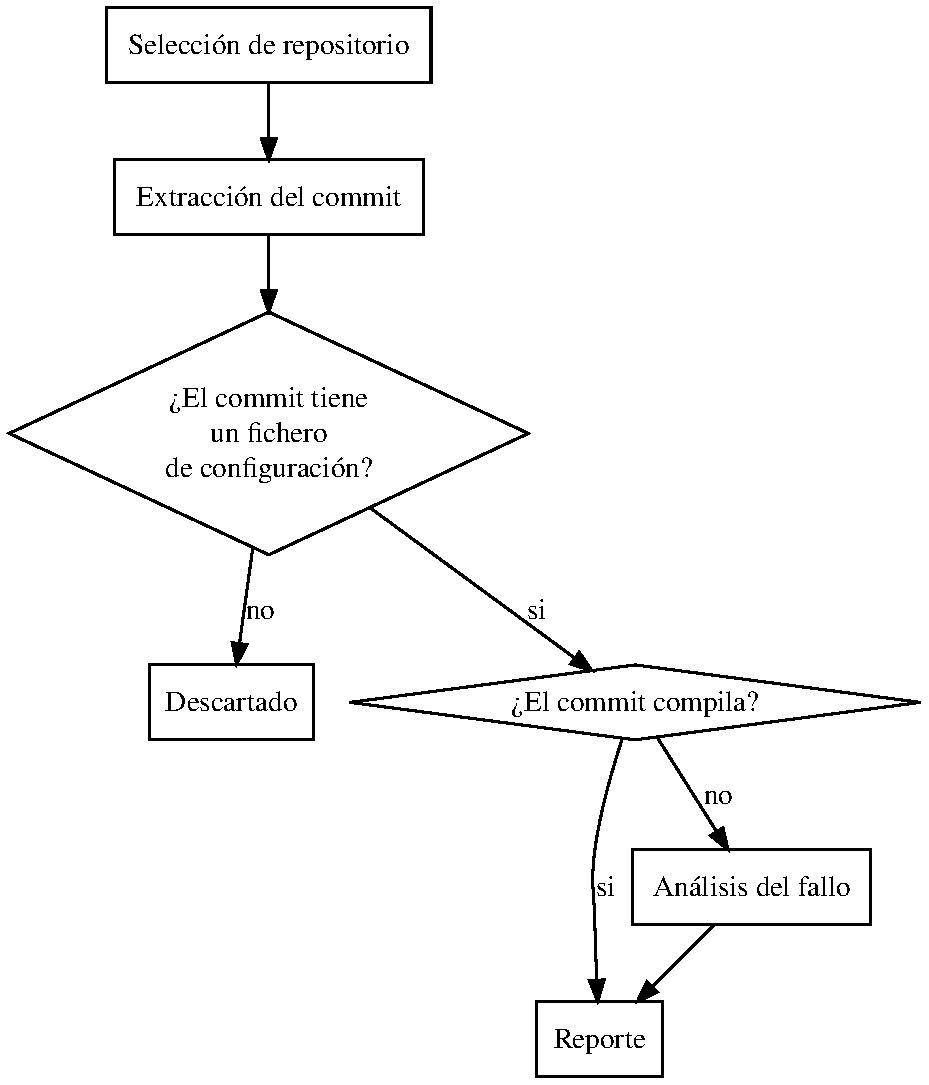
\includegraphics[height=\textwidth]{pages/Appendix/figures/methodology.pdf}
    \caption{Flujo de trabajo básico para los estudios de replicación y reproducción}
    \label{fig:resumen:methodology}
\end{figure}

Este proceso se ejecutará para 79 proyectos Java de Apache (dado que no se pudo recuperar todos los proyectos del estudio original) y 80 proyectos obtenidos de GitHub.

\subsection{Resultados}

Una vez ejecutada la experimentación siguiendo la metodología para los proyectos Apache (replicación) y los proyectos obtenidos de GitHub, obtenemos los siguientes resultados:

\begin{itemize}
    \item \textbf{Replicación}: Pudimos replicar en gran medida el estudio original, descartando un total de 21 proyectos que no pudimos recuperar. 
    Hubo una degradación en la capacidad de construir los commits del proyecto (25.1\%) respecto al experimento original (37.19\%, considerando solo los 79 proyectos disponibles). Esta degradación se debe especialmente por nuevos errores en la compilación derivados de la resolución de dependencias.
    \item \textbf{Reproducción}: En el experimento de reproducción (que contempla otros sistemas de construcción como Ant o Gradle) obtenemos que, de media, podemos construir el 41.66\% de los commits del proyecto. Este valor es muy próximo al del experimento previo original (38\%), además de que la principal razón de fallo en la compilación sigue siendo la resolución de dependencias. Además, comprobamos que el valor medio de commits compilables de un proyecto es sensiblemente mayor si utilizamos Maven (42\%) que si utilizamos Ant (17\%) o Gradle (22\%).
\end{itemize}

\section{Ejecutabilidad de las pruebas en versiones anteriores del código}
\label{sec:resumen:testability}

\subsection{Contexto y objetivos}

La reproducción de programas ejecutables a partir del código fuente de versiones anteriores es fundamental tanto para los profesionales, que necesitan mantener versiones antiguas en producción~\cite{bartelsoftware} o trasplantar a versiones anteriores una funcionalidad con cierta seguridad~\cite{tian2017mining}, como para los investigadores, que necesitan estudiar esas versiones antiguas. 
En la sección anterior se ha estudiado la compilación de versiones anteriores del código fuente de un proyecto.
Sin embargo, no solo la compilación del código fuente es importante, sino que la construcción y ejecución de pruebas de las versiones anteriores también es importante tanto para el mantenimiento como para la investigación.

En este estudio tendremos como objetivo analizar en qué medida se pueden compilar y ejecutar pruebas de versiones pasadas de un proyecto. 
Para ello, seleccionaremos un total de 86 proyectos de Java del conjunto de datos ManySStuBs4J y evaluaremos su testabilidad, definida como la capacidad de ejecutar todas las pruebas con éxito en una version. Este definición viene motivada por los sistemas de integración continua, que ejecutan para una versión del proyecto todas las pruebas y solo la consideran "integrable" esta versión si toda las pruebas pasan.

\subsection{Metodología}

Siguiendo la metodología de la sección anterior, lo ampliaremos, ejecutando los siguientes pasos por cada commit de cada proyecto:

\begin{itemize}
    \item Buscaremos su fichero de configuración. Si lo encuentra, pasaremos al siguiente paso, si no, pasaremos al siguiente commit.
    \item Ejecutaremos el comando de compilación del código fuente.
    \item Ejecutaremos el comando de compilación del código de las pruebas.
    \item Ejecutaremos el comando de ejecución de las pruebas, comprobando si todas las pruebas se ejecutan con éxito.
\end{itemize}

De manera adicional, planteamos un caso de estudio (con un enfoque exploratorio sobre un subconjunto de proyectos) que nos permita comprender cual es la mejor forma de evaluar la testabilidad de un proyecto y si su definición es adecuada.

\subsection{Resultados}

El caso de estudio planteado nos permite concluir que la definición de testabilidad inicialmente definida es muy limitada (una version es apta solo si todas las pruebas pasan). 
Desde el punto de vista de un profesional o un investigador que necesita añadir un cambio a una versión anterior y tiene que evaluar si las pruebas le permiten estar seguro de no introducir ninguna regresión en el código, saber que en un alto porcentaje (pero no el 100\%) de las pruebas pasan puede ser suficiente.
De esta forma, la testabilidad de un proyecto puede ser evaluada de una manera binaria (si todas las pruebas pasan o no) o de una manera más flexible (el porcentaje de pruebas que pasan).

Una vez hemos aplicado la metodología a los 86 proyectos y hemos ampliado la definición de testabilidad, obtenemos los siguientes resultados:

\begin{itemize}
    \item Pudimos compilar el código de los test con un valor medio por proyecto del 41\%. Este valor es muy cercano al de la compilabilidad media del código fuente (47\%). Podemos concluir que cuando el código fuente compila, el por lo que, en general, la compilación de pruebas no es un problema. Sin embargo, los problemas de la compilación del código fuente (siendo un paso previo al de la compilación de los test) son un limitante importante para la experimentación.
    \item Considerando la testabilidad en su forma binaria (todos los test pasan o no), obtenemos que, de media, en el 22\% de las versiones de un proyecto podemos ejecutar todas sus pruebas con éxito. Si consideramos solo las versiones en las que somos capaces de compilar las pruebas, este porcentaje aumenta considerablemente (52\%).
    \item Considerando la testabilidad como el porcentaje de pruebas que pasan en una version, obtenemos que, de media, para las versiones del un proyecto, el 38\% de las pruebas pasan con éxito. Si consideramos solo las versiones en las que somos capaces de compilar las pruebas, este porcentaje aumenta considerablemente (94\%). 
\end{itemize}


\section{Localización del cambio que introdujo el error a través de las pruebas de regresión}
\label{sec:resumen:bug-hunter}

\subsection{Contexto y objetivos}

Los errores son una de las principales preocupaciones de los desarrolladores de software. 
Encontrar errores en el código y corregirlos consume mucho esfuerzo. 
Aprender cómo se introdujeron los errores es importante tanto para los académicos como para los profesionales. 
Los profesionales desean saber qué cambio introdujo un error cuando intentan corregirlo y qué versiones anteriores se ven afectadas por él. 
Los investigadores quieren estudiar cómo se introdujeron los error para encontrar formas de prevenirlos. 
Sin embargo, encontrar el cambio de código fuente que introdujo el error no es fácil.

Hay variar propuestas que intentan detectar automáticamente estos cambios que introducen el error. 
El estado del arte más reconocido en este campo es el SZZ~\cite{sliwerski2005changes}, un algoritmo basado en la identificación del cambio que corrige el error para analizar las líneas que han sido modificadas o eliminadas, asumiendo que el último cambio realizado en esas líneas antes de la corrección fue el cambio que introdujo el error.
Sin embargo, el algoritmo se ve limitado cuando la premisa no se cumple.
Como consecuencia, Rodríguez et al.~\cite{rodriguez2020bugs} propone el método de la "prueba perfecta", que proponía un enfoque completamente diferente al SZZ y pretendía mitigar las limitaciones de este algoritmo. 
El método de la prueba perfecta es una construcción teórica cuyo objetivo es detectar cambios que introducen errores (en inglés
Bug Introduction Changes o BICs) a través de un prueba perfecta teórica.
Esta prueba perfecta siempre falla si el error está presente, y pasa en caso contrario. En teoría, esta prueba perfecta permitiría detectar el error en el historial de cambios de un proyecto.

En este estudio tendremos como objetivo operacionalizar el método de la prueba perfecta para poder aplicarlo a proyectos de software reales.
Es una práctica común en el desarrollo de software que, cuando se detecta y corrige un error, los desarrolladores escriban una
prueba que detecte dicho error en caso de que reaparezca, lo que se conoce como una prueba de regresión. 
Esta prueba puede incluso estar disponible como parte del informe de error antes de que se corrija el error (la corrección está dirigida por pruebas).
Planteamos por lo tanto la hipótesis de que las pruebas de regresión podrían utilizarse como pruebas perfectas para detectar el cambio que introdujo el error

\subsection{Metodología}

Para evaluar la hipótesis, se ha desarrollado una herramienta que utiliza las pruebas de regresión para detectar el cambio que introdujo el error.
Para evaluar la herramienta y por tanto la hipótesis, utilizaremos un conjunto de 809 errores localizados en 16 proyectos de un popular dataset de proyectos Java (Defects4J~\cite{just2014defects4j}).
La herramienta sigue los siguientes pasos para cada error:
\begin{itemize}
    \item Extrae la información del error: el cambio que arregla del error, la prueba de regresión escrita junto ese cambio y el reporte de error.
    \item Clona el repositorio de código
    \item Ejecuta la prueba de regresión en el cambio que arregla el error, comprobando que la prueba pasa con éxito.
    \item Ejecuta la prueba de regresión en los cambios previos al cambio que arregla el error. 
\end{itemize}

Por cada cambio, se ejecutarían los siguientes pasos:
\begin{inparaenum}[\bf(1)]
    \item nos situamos en el cambio que queremos probar,
    \item trasplantamos (copiamos) la prueba de regresión,
    \item compilamos el código fuente,
    \item ejecutamos la prueba de regresión,
    \item ejecutamos la prueba de regresión y
    \item recopilamos el resultado de la prueba.
\end{inparaenum}

Para localizar el cambio que introdujo el error, consideramos el histórico de cambios como un grafo dirigido que parte del cambio que arregla el error y va hacia atrás en el tiempo. 
Recorriendo este grafo encontraremos 2 posibles casos:
\begin{itemize}
    \item Encontramos un cambio donde la prueba falla, pero los cambios directamente anteriores a este cambio pasan la prueba. En este caso, el cambio que falla es el cambio que introdujo el error. Es posible que encontremos casos donde la prueba vuelve a pasar con éxito pero el cambio siguiente es uno dónde la prueba no puede ser ejecutada (por ejemplo, porque no se puede compilar el código fuente o de los test). En este caso, todos los commits siguientes hasta el primero en el que si se pueda ejecutar la prueba y falle son candidatos a ser el cambio que introdujo el error.
    \item No encontramos ningún cambio donde la prueba vuelve a pasar, por lo que asumimos que el cambio estuvo siempre en el código o no fuimos capaces de trasplantar la prueba lo suficientemente lejos en el pasado.
\end{itemize}

Aplicando los conocimientos adquiridos en los estudios anteriores, utilizaremos medidas de mitigación para los problemas que impiden la compilación del código fuente o la ejecución de la prueba de regresión.

Una vez detectados los cambios que introdujeron el error, validaremos de manera manual los resultados obtenidos con el fin de comprobar la fiabilidad de la herramienta y para generar un nuevo conjunto de datos que pueda ser utilizado por otros investigadores.

\subsection{Resultados}

Tras aplicar la herramienta desarrollada a los 809 errores de los 16 proyectos de Defects4J, se obtuvieron los siguientes resultados:

\begin{itemize}
    \item Se comprobó que para los 809 errores, la prueba de regresión pudo ser trasplantada y ejecutada en el 33\% de los cambios del historial de cambios.
    Encontramos que la principal causa de que la prueba no pudiera ser ejecutada era que el código fuente no podía ser compilado, problema parcialmente mitigado por la herramienta desarrollada gracias a el conocimiento adquirido en el estudio de la compilabilidad del software.
    \item De los 809 errores, la herramienta encontró un cambio dónde la prueba de regresión vuelve a pasar con éxito en 96 casos. En 67 casos se encontró un único candidato a ser el cambio que introdujo el, mientras que en 29 casos se encontraron varios candidatos.
    \item De los 67 casos dónde se encontró un candidato, se comprobó manualmente que era el cambio que introdujo el error. 
    Como resultado, generamos un conjunto de datos con estos 67 errores y el cambio que introdujo el error, que puede ser utilizado por otros investigadores.
    \item Los errores son esencialmente introducidos en un cambio que pretende solucionar otro error o mediante una refactorización o reimplementación.
\end{itemize}

\section{Conclusiones y trabajos futuros}
\label{sec:resumen:conclusiones}

En esta tesis se han estudiado en detalle dos propiedades de la evolución del software: la compilabilidad del software en sus versiones pasadas y la capacidad de ejecutar pruebas también en versiones anteriores del código. 
Además, a partir de lo aprendido en estos estudios, se ha propuesto una herramienta para detectar el cambio que introdujo un error en el código haciendo uso del historial de cambios y de las pruebas de regresión. 

En el Capítulo~\ref{chapter:buildability}, se llevó a cabo un estudio de replicación y reproducción del trabajo de Tufano et al.~\cite{tufano2017there} sobre la compilabilidad de la historia de los commits anteriores de un proyecto. Los resultados obtenidos incluyen pautas y directrices para paquetes de reproducción, un conjunto de datos y software para estudiar la degradación a largo plazo de la compilabilidad, y evidencia sobre cómo la compilabilidad se degrada con el tiempo y cómo se puede mitigar. 
En el Capítulo~\ref{chapter:testability}, se realizó un análisis empírico de la capacidad de prueba de versiones pasadas de proyectos, y se propuso un marco para analizar esto en el futuro. El alto grado de variabilidad en la capacidad de prueba se encontró en la mayoría de las versiones. 
En el Capítulo~\ref{chapter:bug-hunter}, se propuso la operacionalización de un método teórico para detectar el cambio que introdujo un error a través de pruebas de regresión. 
Se generó, además, un conjunto de datos de manera automática de estos los cambios localizados, que se pueden utilizar para evaluar otros métodos que detectan los cambios que introdujeron errores.

A lo largo de este proyecto de investigación, se ha generado un artículo publicado en la revista \textit{Empirical Software Engineering}, situada en el el primer cuartil (Q1) de su campo, correspondiente al Capitulo~\ref{chapter:buildability}. 
El Capítulo~\ref{chapter:testability} está planteado como publicación en la revista \textit{Software Evolution and Process}. 
Por último, la investigación recogida en el Capítulo~\ref{chapter:bug-hunter} ha sido mandada a la revista \textit{Empirical Software Engineering} y se encuentra en proceso de revisión.

La tesis doctoral presentada se limita a proyectos escritos en el lenguaje de programación Java, mayormente librerías de programación cuya mayoría de pruebas son unitarias. Por lo tanto, se necesitan más investigaciones para extraer conclusiones generales sobre la compilabilidad y prueba de versiones pasadas, identificar cambios que introdujeron errores y aplicarlo a otros lenguajes de programación y proyectos con diferentes prácticas de prueba. En el Capítulo~\ref{chapter:testability}, se destaca la limitación de no tener acceso a la información de compilación y ejecución de pruebas de versiones pasadas debido a la falta de sistemas de integración continua accesibles públicamente. 
Por lo tanto, un posible trabajo futuro sería crear un nuevo conjunto de datos de construcciones y ejecuciones de pruebas que nos ayuden a comprender cómo se comportaban las pruebas en el momento momento en que se ejecutaron y en el contexto adecuado.
En el Capítulo~\ref{chapter:bug-hunter}, se propone una herramienta para buscar exhaustivamente el cambio que introdujo un error, pero esta herramienta también tiene limitaciones debido a la dificultad para reproducir el contexto de prueba y al tiempo requerido para calcular los resultados de ejecución de prueba en la historia de cambios. Se plantea una investigación futura que combine la herramienta propuesta con las últimas implementaciones de SZZ para mejorar su eficacia.